\chapter{Introducci�n a redes neuronales}

\hline

Las Redes Neuronales Artificiales (ANNs de Artificial Neural Networks) fueron originalmente una simulaci�n abstracta de los sistemas nerviosos biol�gicos, formados por un conjunto de unidades llamadas "neuronas" o "nodos" conectadas unas con otras. Estas conexiones tienen una gran semejanza con las dendritas y los axones en los sistemas nerviosos biol�gicos. 

El Primer modelo de red neuronal fue propuesto en 1943 por McCulloch y Pitts en t�rminos de un modelo computacional de "actividad nerviosa". El modelo de McCulloch-Pitts es un modelo binario, y cada neurona tiene un escal�n o umbral prefijado. Este primer modelo sirvi� de ejemplo para los modelos posteriores de Jhon Von Neumann, Marvin Minsky, Frank Rosenblatt, y muchos otros. 

Pongamos de ejemplo el cerebro humano:
\begin{itemize}
\item Formado por una red de neuronas interconectadas.
\item 10^{10} neuronas en el cerebro humano.
\item Tiempo de conmutaci�n 0,001 segundo (computadora: 10^{-10}).
\item Tiempo que se tarda en reconocer una imagen: 0.1 segundo.
\item 100 pasos de procesamiento parecen pocos para resolver un problema tan complejo como el reconocimiento de im�genes.
\item Hip�tesis: el cerebro humano presenta un paralelismo masivo sobre una representaci�n distribuida.
\end{itemize} 	

Debido a la inspiraci�n ya mencionada de las ANN en el cerebro, sus aplicaciones principales estar�n centradas en campos donde la inteligencia humana no pueda ser emulada de forma satisfactoria por algoritmos aritm�ticos que pueden ser implementados en ordenadores. Adem�s es de prever que dichas ANN tengan caracter�sticas similares a las del cerebro: 
\begin{itemize}
\item Ser�n robustas i tolerantes a fallos. En el cerebro mueren todos los d�as gran cantidad de neuronas sin afectar sensiblemente a su funcionamiento.
\item Ser�n flexibles. El cerebro se adapta a nuevas circunstancias mediante el aprendizaje .
\item Podr�n trabajar con informaci�n borrosa, incompleta, probabil�stica, con ruido o inconsistente. 
\item Ser�n altamente paralelas. El cerebro esta formado por muchas neuronas interconectadas entre si y es precisamente el comportamiento colectivo de todas ellas lo que caracteriza su forma de procesar la informaci�n.
\end{itemize} 
Resumiendo una ANN es un gran numero de conmutadores interconectados, donde a las conexiones se les asigna un peso. Este peso ser� fijado durante la fase de aprendizaje. El procesamiento de informaci�n es paralelo distribuido.

En que tipos de problemas se utilizan:
\begin{itemize}
\item En problemas donde los ejemplos se describen con un gran numero de atributos.
\item Puede haber ruido en los datos.
\item Cuando no se conoce la forma de la funci�n objetivo. Problemas que no tienen un algoritmo especifico para su soluci�n, o cuyo algoritmo es demasiado complejo para ser encontrado. 
\item Cuando es permisible un tiempo de entrenamiento largo.
\item Ejemplos: Reconocimiento del habla, clasificaci�n de im�genes, predicciones financieras, etc.
\end{itemize} 

\begin{center}
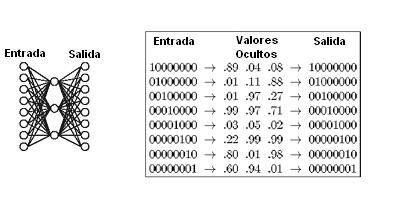
\includegraphics[scale=1]{red1.png} 
Ejemplo grafico de una red.
\end{center} 

Existen dos fases en toda aplicaci�n de las redes neuronales: la fase de aprendizaje o entrenamiento y la fase de prueba. En la fase de entrenamiento, se usa un conjunto de datos o patrones de entrenamiento para determinar los pesos (par�metros de dise�o) que definen el modelo neuronal. Una vez entrenado este modelo, se usar� en la llamada fase de prueba o funcionamiento directo, en la que se procesan los patrones de prueba que constituyen la entrada habitual de la red, analiz�ndose de esta manera las prestaciones definitivas de la red.

En general, las Redes Neuronales Artificiales han sido claramente aceptadas como nuevos sistemas muy eficaces para el tratamiento de la informaci�n en muchas disciplinas. Ellos ha dado como resultado una variedad de aplicaciones comerciales (tanto en productos como en servicios) de esta tecnolog�a de redes neuronales.

